\begin{figure}
    \centering
    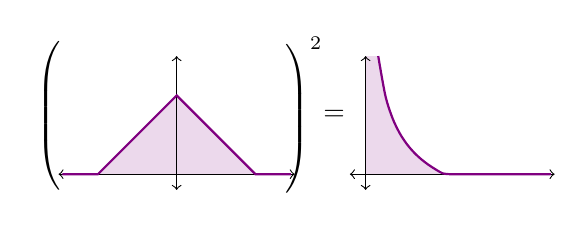
\begin{tikzpicture}
        \fill[Purple!15] (-1, 0) -- (0, 1) -- (1, 0) -- cycle;

        \draw[<->] (-1.5, 0) -- (1.5, 0);
        \draw[<->] (0, -0.2) -- (0, 1.5);

        \draw[Purple, thick] (-1.45, 0) -- (-1, 0) -- (0, 1) -- (1, 0) -- (1.45, 0);

        \node at (-1.6, 0.75) {\( \left(\rule{0pt}{30pt} \right. \)};
        \node at (1.6, 0.75) {\( \left. \rule{0pt}{30pt} \right)^2 \)};

        \node at (2.0, 0.75) {\( = \)};

        \fill[color=Purple!15, thick, domain=0.16:1] plot ({\x + 2.4}, {1/sqrt(\x) - 1}) -- (2.4,0) -- (2.4, 1.5) -- cycle;

        \draw[<->] (2.2, 0) -- (4.8, 0);
        \draw[<->] (2.4, -0.2) -- (2.4, 1.5);

        \draw[Purple, thick] (3.4, 0) -- (4.75, 0);
        \draw[color=Purple, thick, domain=0.16:2.35, smooth] plot ({\x + 2.4}, {(1/sqrt(\x) - 1) * (\x <= 1) + (\x > 1) * (0)});
    \end{tikzpicture}
    \caption{The distribution of the squares of the differences in components.
    It looks rather interesting as it approaches infinity on one side.}
    \label{013:tsquared}
\end{figure}
